\textbf{\textit{Toutes les réponses de cet exercice devront être justifiées.}}

\bigskip
\begin{minipage}[t]{.5\linewidth}
	On considère la figure ci-contre constituée d’un carré de côté 8 cm dans lequel sont inscrits deux demi-cercles de diamètre un côté du carré.
\end{minipage}
\begin{minipage}{.5\linewidth}
	\centering
	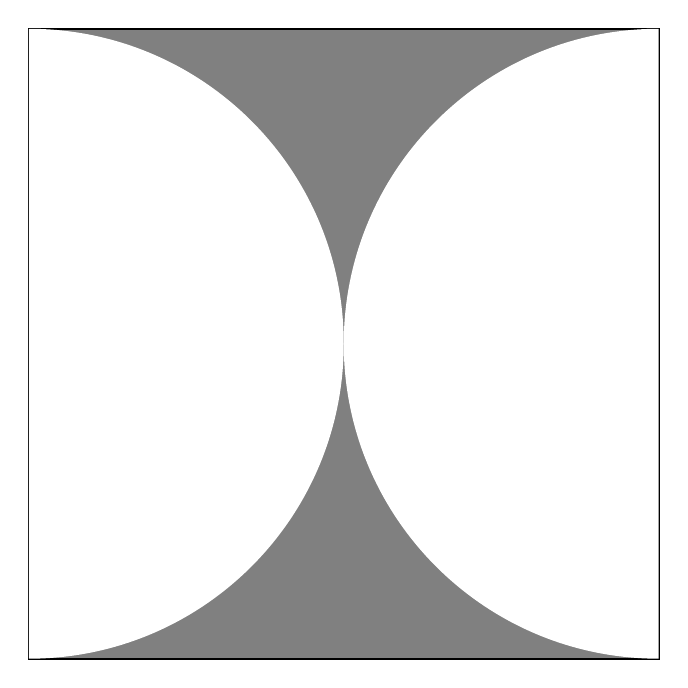
\begin{tikzpicture}
    	\fill[gray] (0,0) rectangle (8,8); % Remplit un carré de 8 cm en gris
    	\draw[black,thick] (0,0) rectangle (8,8); % Dessine un carré de 8 cm avec des bords noirs et épais
    	\fill[thick,white] (0,0) arc[start angle=-90, end angle=90, radius=4cm]; % Dessine un demi-cercle blanc en bas
	    \fill[thick,white] (8,8) arc[start angle=90, end angle=270, radius=4cm]; % Dessine un demi-cercle blanc en haut
	\end{tikzpicture}
\end{minipage}

\begin{enumerate}
	\item Déterminer l'aire du carré.
	\item Déterminer la valeur exacte de l'aire grisée en cm\up{2}.
	\item On souhaite reproduite cette figure sur le sol d'une cour de récréation à l'échelle 125 : 1.
	\begin{enumerate}
		\item Quel sera le côté du nouveau carré ? Exprimer le résultat en mètre.
		\item Quelle sera la dimension de la diagonale de ce nouveau carré ? Donner le résultat en mètre arrondi au cm. 
	\end{enumerate}
	
	\item On souhaite peindre la zone grisée de deux couches de peinture. Sachant que le rendement de la peinture est de 7~m\up{2}/L et se vend par pot de 750~mL, combien de pots de peinture faut-il prévoir ?

\end{enumerate}